
\chapter{Geometric and topological nature of cut locus}\label{ch:GeometricViewpointOfCutLocus}
\minitoc
\hf The objective of this chapter is to analyze the geometric and topological properties of cut locus of submanifolds. In particular, we will study relations between the distance squared function from a submanifold, the cut locus of submanifold and Thom space of the normal bundle of the submanifold. We will also prove that the distance squared function is a Morse-Bott function. Results in this chapter are based on joint work with Basu \cite{BaPr21}.

\hf A result due to Wolter \cite[Lemma 1]{Wol79} may be generalized to prove (\Cref{Lmm: singdsq}) that the distance squared function from a submanifold is not differentiable on the separating set. This result may be well known to experts, but we provide a proof, following Wolter, which is elementary.

\section{Regularity of distance squared function}\label{sec:RegularityOfDistanceSquaredFunction}
\hfb Recall \Cref{defn:DeltaMap}, where we have defined the $\Delta$ map. The following proposition describes $\Delta$ in terms of the distance function on the Riemannian manifold $M$ from the submanifold $N$.

\vspace{0.3cm}
\begin{prop}\label{dsq-Fermi}
    Let $U$ be a neighbourhood of $N$ such that each point in $U$ admits a unique unit speed $N$-geodesic. If $p\in U$, then 
    \begin{displaymath}
        \Delta(p) = \dist(N,p).
    \end{displaymath}
\end{prop}
\vspace{0.1cm}
\begin{proof}
    Since the expression of $\Delta$ is independent of the choice of the Fermi coordinates, we will make a special choice of the Fermi coordinates $(x_1,\cdots,x_n)$. For $p\in U$, choose the unique unit speed $N$-geodesic $\gamma$ joining $p$ to $N$. This geodesic meets $N$ orthogonally at $\gamma(0)=p'$. Choose $t_0$ such that $\gamma(t_0)= p$.
    \begin{figure}[!htpb]
        \centering
        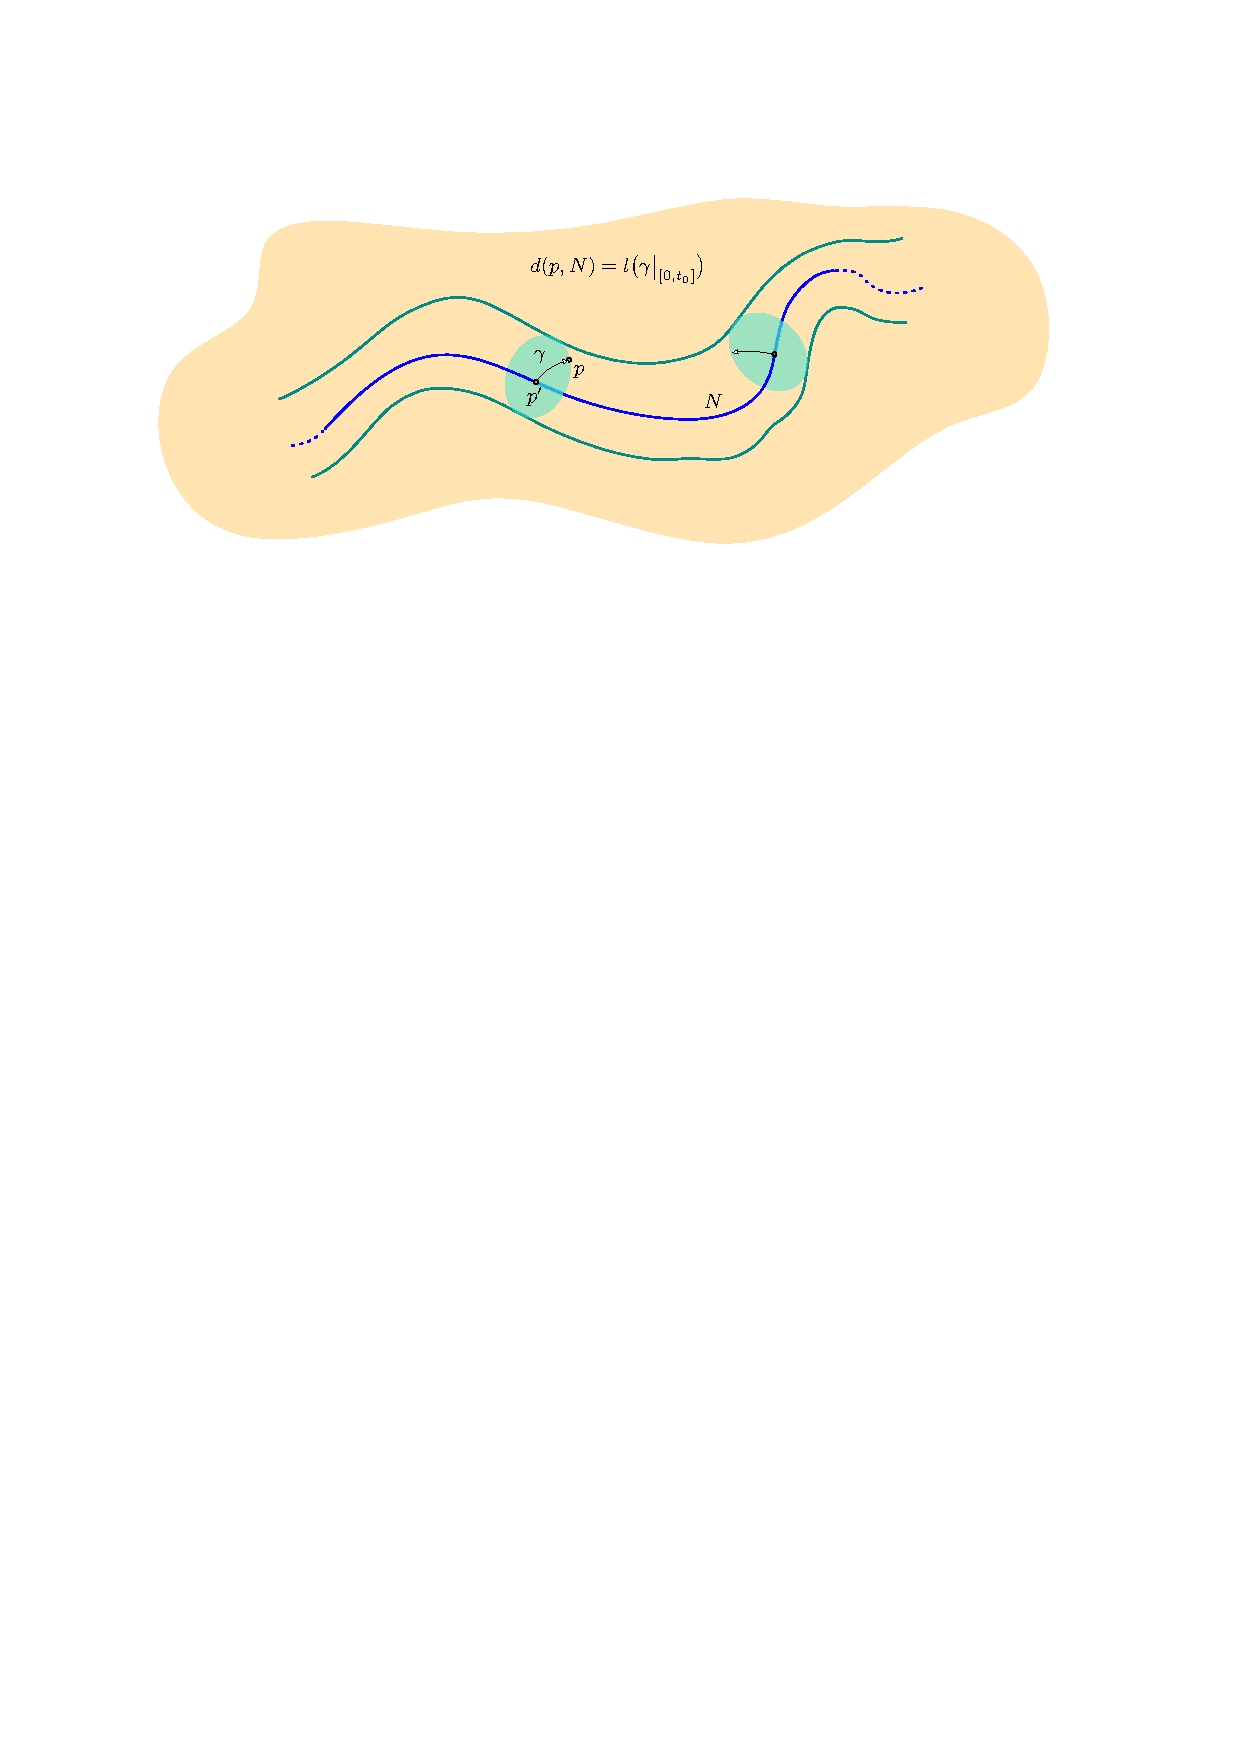
\includegraphics[width=0.85\textwidth]{figures/Fermi.pdf}
        \caption{Distance via Fermi coordinates}
        \label{fig:distancesquared}
    \end{figure}
    \noindent According to \autoref{Lemma: geodesic in fermi}, there is a system of Fermi coordinates $(x_1,\cdots,x_n)$ centered at $p'$ such that $x_i(\gamma(t)) = t\delta_{i(k+1)}$. The sequence of equalities 
    \begin{displaymath}
        \Delta(p) = x_{k+1}(\gamma(t_0)) = t_0 = \dist(p,N)
    \end{displaymath}
    complete the proof.
\end{proof}

\begin{cor}\label{dsq-MB}
    Consider the distance squared function with respect to a submanifold $N$ in $M$. The Hessian of the distance squared function at the critical submanifold $N$ is non-degenerate in the normal direction. 
\end{cor}

\vspace{0.3cm}
\hf Towards the regularity of distance squared function, the following observation will be useful. It is a routine generalization of \cite[Lemma~1]{Wol79}.

\begin{lemma}\cite[Lemma 3.7]{BaPr21} \label{Lmm: singdsq}
    Let $M$ be a connected, complete Riemannian manifold and $N$ be an embedded submanifold of $M$. Suppose two $N$-geodesics exist joining $N$ to $q\in M$. Then $d^2(N,\cdot):M\to \rbb$ has no directional derivative at $q$ for vectors in direction of those two $N$-geodesics. 
\end{lemma}
\begin{proof}
    Let us assume that all the geodesics are arc-length parametrized. Let $\gamma_i:[0,\hat{t}]\to M,~~i=1,2$,  be two distinct geodesics with $\gamma_1(0), \gamma_2(0)\in N$ and $\gamma_1(l)=q=\gamma_2(l)$, where $l=d(N,q)$ and $0<l<\hat{t}$. Suppose that the two geodesics start at $p_1$ and $p_2$ and so $d(p_1,q)=l=d(p_2,q)$. Note that the directional derivative of $d^2$ at $q$ in the direction of $\gamma_i'(q)$ from the left is given by
    \begin{align*}
        (d^2)'_-(q) & := \lim_{\varepsilon\to 0^+} \dfrac{(d(N,\gamma_i(l)))^2-(d(N,\gamma_i(l-\varepsilon)))^2}{\varepsilon}\\
		& = \lim_{\varepsilon\to 0} \dfrac{(d(p_i,\gamma_i(l)))^2-(d(p_i,\gamma_i(l-\varepsilon)))^2}{\varepsilon}\\
        & = \lim_{\varepsilon\to 0^+} \dfrac{l^2-(l-\varepsilon)^2}{\varepsilon}\\
		& = \lim_{\varepsilon\to 0} \dfrac{l^2-l^2+2l\varepsilon-\varepsilon^2}{\varepsilon}\\
		& = \lim_{\varepsilon\to 0}\dfrac{2l\varepsilon-\varepsilon^2}{\varepsilon}\\
        & = 2l.
    \end{align*}
    Next, we claim that the derivative of the same function from the right is strictly bounded above by $2l$. Let $\omega\in(0,\pi]$ be the angle between the two geodesics $\gamma_1$ and $\gamma_2$ at $q$.  Define the function,
    \begin{equation*}
        u(\tau)\defeq d(N,\gamma_1(l-\varepsilon))+d(\gamma_1(l-\varepsilon),\gamma_2(\tau+l)).
    \end{equation*} 
    \begin{figure}[h]
        \centering
        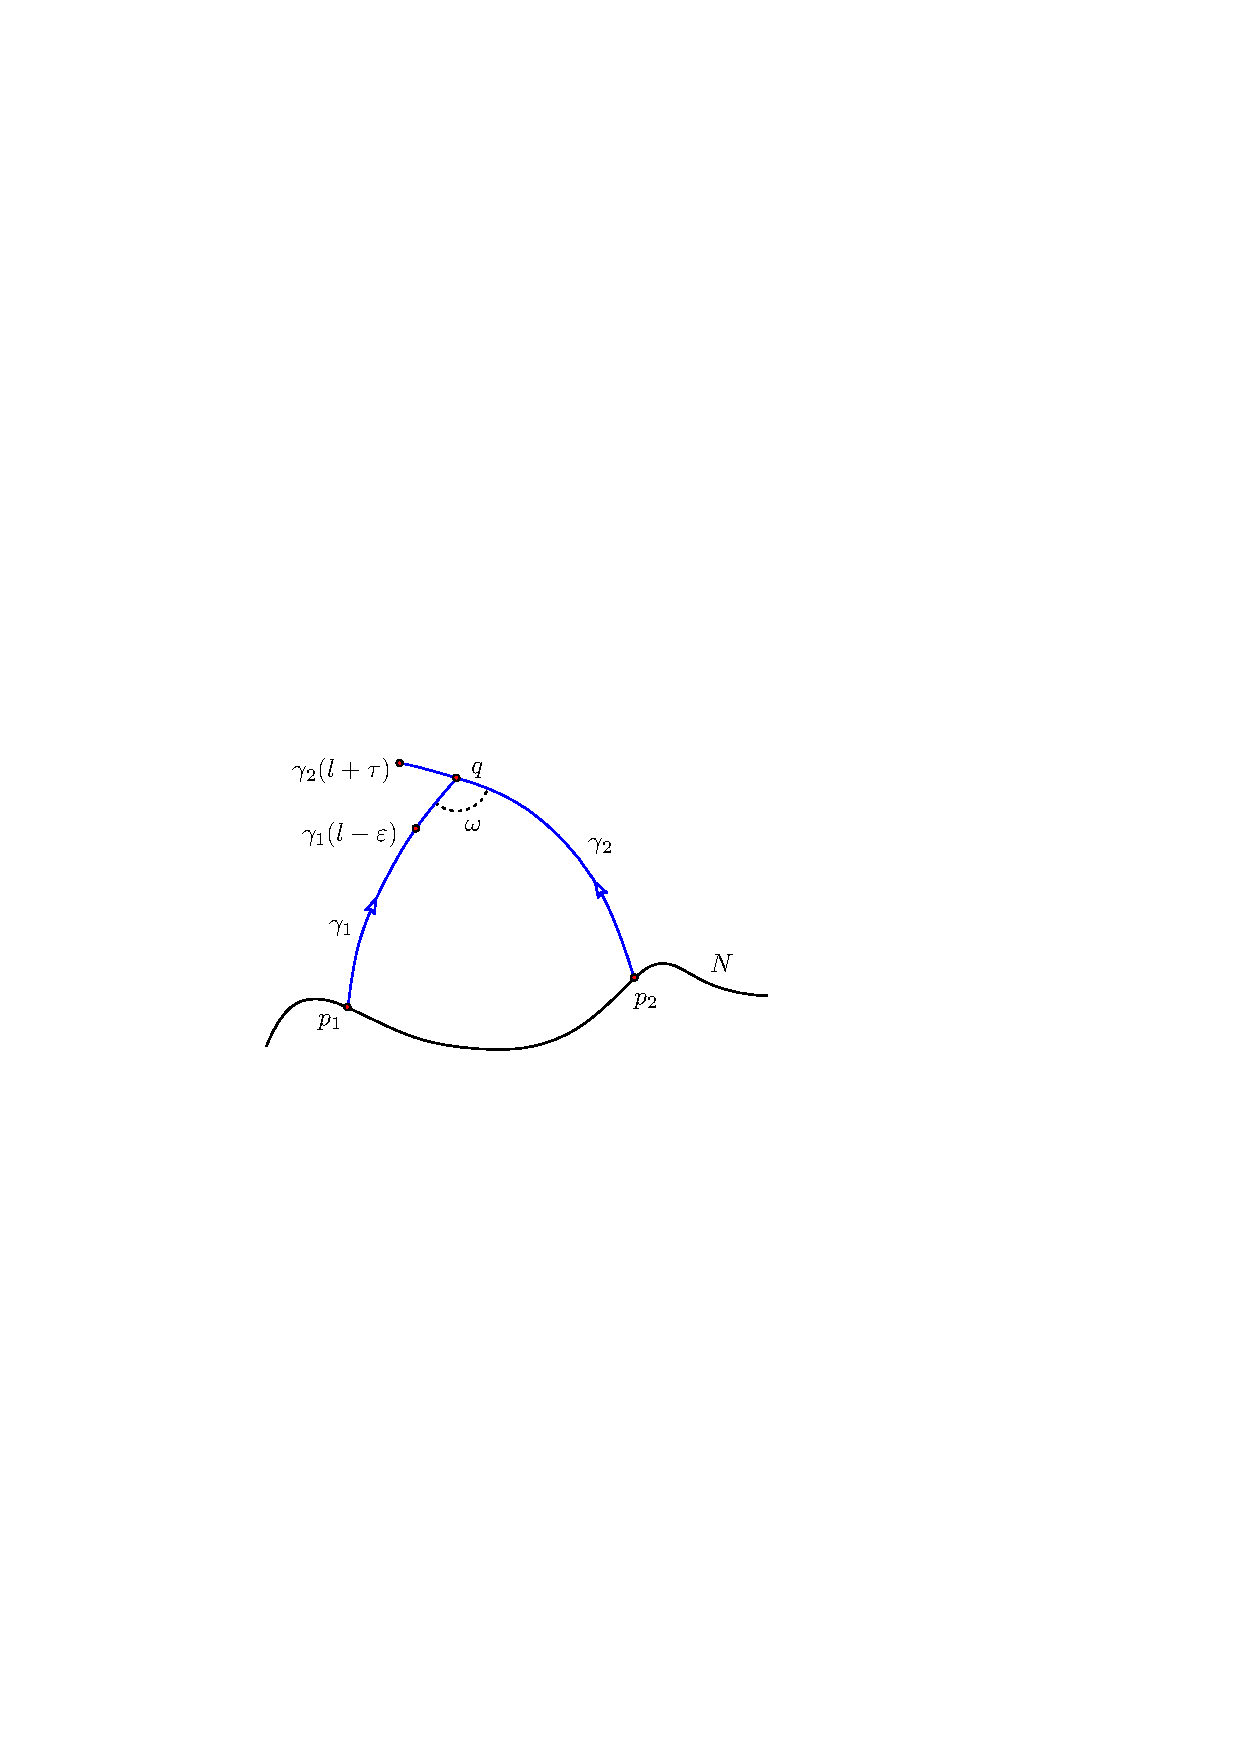
\includegraphics[scale=1]{Se_N.pdf}
        \caption{When two $N$-geodesics meet}
        \label{fig: notDifferentiable}
    \end{figure}
    By triangle inequality, we observe that
    \begin{equation*}
    f(\tau)\defeq (u(\tau))^2 \ge d^2(p_1,\gamma_2(\tau+l)) \ge d^2(N,\gamma_2(\tau+l)),
    \end{equation*}
    and equality holds at $\tau=0$ and $(u(0))^2=d^2(N,q)=l^2$. Thus, in order to prove the claim, it suffices to show that the derivative of $f$ from right, at $\tau=0$, is bounded below by $2l$. We need to invoke a version of the cosine law for small geodesic triangles. Although this may be well-known to experts, we will use the version that appears in \cite{Sha07} (also see \cite[Lemma 2.4]{DaDe18} for a detailed proof). In our case, this means that 
    \begin{displaymath}
        d^2(\gamma_1(l-\varepsilon),\gamma_2(\tau+l))=\ep^2+\tau^2+2\ep\tau \cos \omega +K(\tau)\ep^2\tau^2
    \end{displaymath}
    where $|K(\tau)|$ is bounded, and the side lengths are sufficiently small. Note that we are considering geodesic triangles with two vertices constant and the varying vertex being $\gamma_2(l+\tau)$. It follows from taking a square root and then expanding in powers of $\tau$ that
    \begin{displaymath}
        d(\gamma_1(l-\varepsilon),\gamma_2(\tau+l))=\sqrt{\varepsilon^2+\tau^2+2\varepsilon\tau\cos\omega}~(1+O(\tau^2)).
    \end{displaymath}
    It follows that 
    \begin{displaymath}
        u(\tau)=l-\ep+\sqrt{\varepsilon^2+\tau^2+2\varepsilon\tau\cos\omega}~(1+O(\tau^2)).
    \end{displaymath} 
    Therefore, $u'_+(0)=\cos \omega=d'_+(\gamma_1(l-\varepsilon),\gamma_2(l))$. Observe that 
    \begin{align*}
        f'_+(\tau)\Big|_{\tau=0} & = 2d(N,\gamma_1(l-\varepsilon))d'_+(\gamma_1(l-\varepsilon),\gamma_2(l)) \\
        & \kern 3cm +2d(\gamma_1(l-\varepsilon),\gamma_2(l))d'_+(\gamma_1(l-
    \varepsilon),\gamma_2(l))\\
        & = 2d(N,\gamma_1(l-\varepsilon))\cos \omega+2d(\gamma_1(l-\varepsilon),\gamma_2(l))\cos\omega\\
		& = 2\cos \omega\big[ d(N,\gamma_1(l-\varepsilon))+d(\gamma_1(l-\varepsilon),\gamma_2(l))) \big]\\
		& = 2\cos\omega \big[ d(N,\gamma_1(l-\varepsilon))+d(\gamma_1(l-\varepsilon),\gamma_1(l))) \big] \\
        & =2d(N,\gamma_1(l))\cos\omega<2l.
    \end{align*}
    Thus, we have proved the claim and subsequently the result.
\end{proof}

\hf The above lemma shows that $d^2$ is smooth away from the cut locus. The following example suggests that $d^2$ can be differentiable at points in $\cutn -\sen$ (see \Cref{defn:SeparatingSet}) but not twice differentiable.

\vspace{0.3cm}
\begin{eg}[Cut locus of an ellipse]\label{eg:CutLocusOfEllipse-2}
    We discuss the regularity of the distance squared function from an ellipse $x^2/a^2+y^2/b^2=1$ (with $a>b>0$) in $\R^2$. For a discussion of the cut locus for ellipses inside $\mathbb{S}^2$ and ellipsoids, see \cite[pages 90-91]{Heb95}. Let $(x_0,y_0)$ be a point inside the ellipse lying in the first quadrant. The point closest to $(x_0,y_0)$ and lying on the ellipse is given by 
    \begin{displaymath}
        x=\frac{a^2x_0}{t+a^2},\,\,y=\frac{b^2y_0}{t+b^2},
    \end{displaymath}
    where $t$ is the unique root of the quartic
    \begin{displaymath}
        \left(\frac{ax_0}{t+a^2}\right)^2+\left(\frac{by_0}{t+b^2}\right)^2=1
    \end{displaymath}
    in the interval $(-b^2,\infty)$. Given $(\alpha,\beta)$ with $\beta>0$, we set $P_\ep(\alpha,\beta)=(\frac{a^2-b^2}{a}+\ep\alpha,\ep\beta)$; this defines a straight line passing through $P_0(\alpha,\beta)$ in the direction of $(\alpha,\beta)$. For $\ep>0$, $P_\ep(\alpha,\beta)$ lies in the first quadrant and we denote by $t=t(\ep)$ be the unique relevant root of the quartic
    \begin{displaymath}
        \left(\frac{a(\frac{a^2-b^2}{a}+\ep\alpha)}{t+a^2}\right)^2+\left(\frac{b\ep\beta}{t+b^2}\right)^2=1.
    \end{displaymath}
    Simplifying this after dividing by $\ep$ and taking a limit $\ep\to 0^+$, we obtain
    \begin{displaymath}
        \frac{2a\alpha}{a^2-b^2}=\lim_{\ep\to 0^+}\left(\Big(\frac{2}{a^2-b^2}\Big)\frac{t+b^2}{\ep}-b^2\beta^2 \frac{\ep}{(t+b^2)^2}\right).
    \end{displaymath}
    On the other hand, the point $Q_\ep(\alpha,\beta)$ on the ellipse closest to $P_\ep(\alpha,\beta)$ is given by
    \begin{figure}[!htpb]
        \centering
        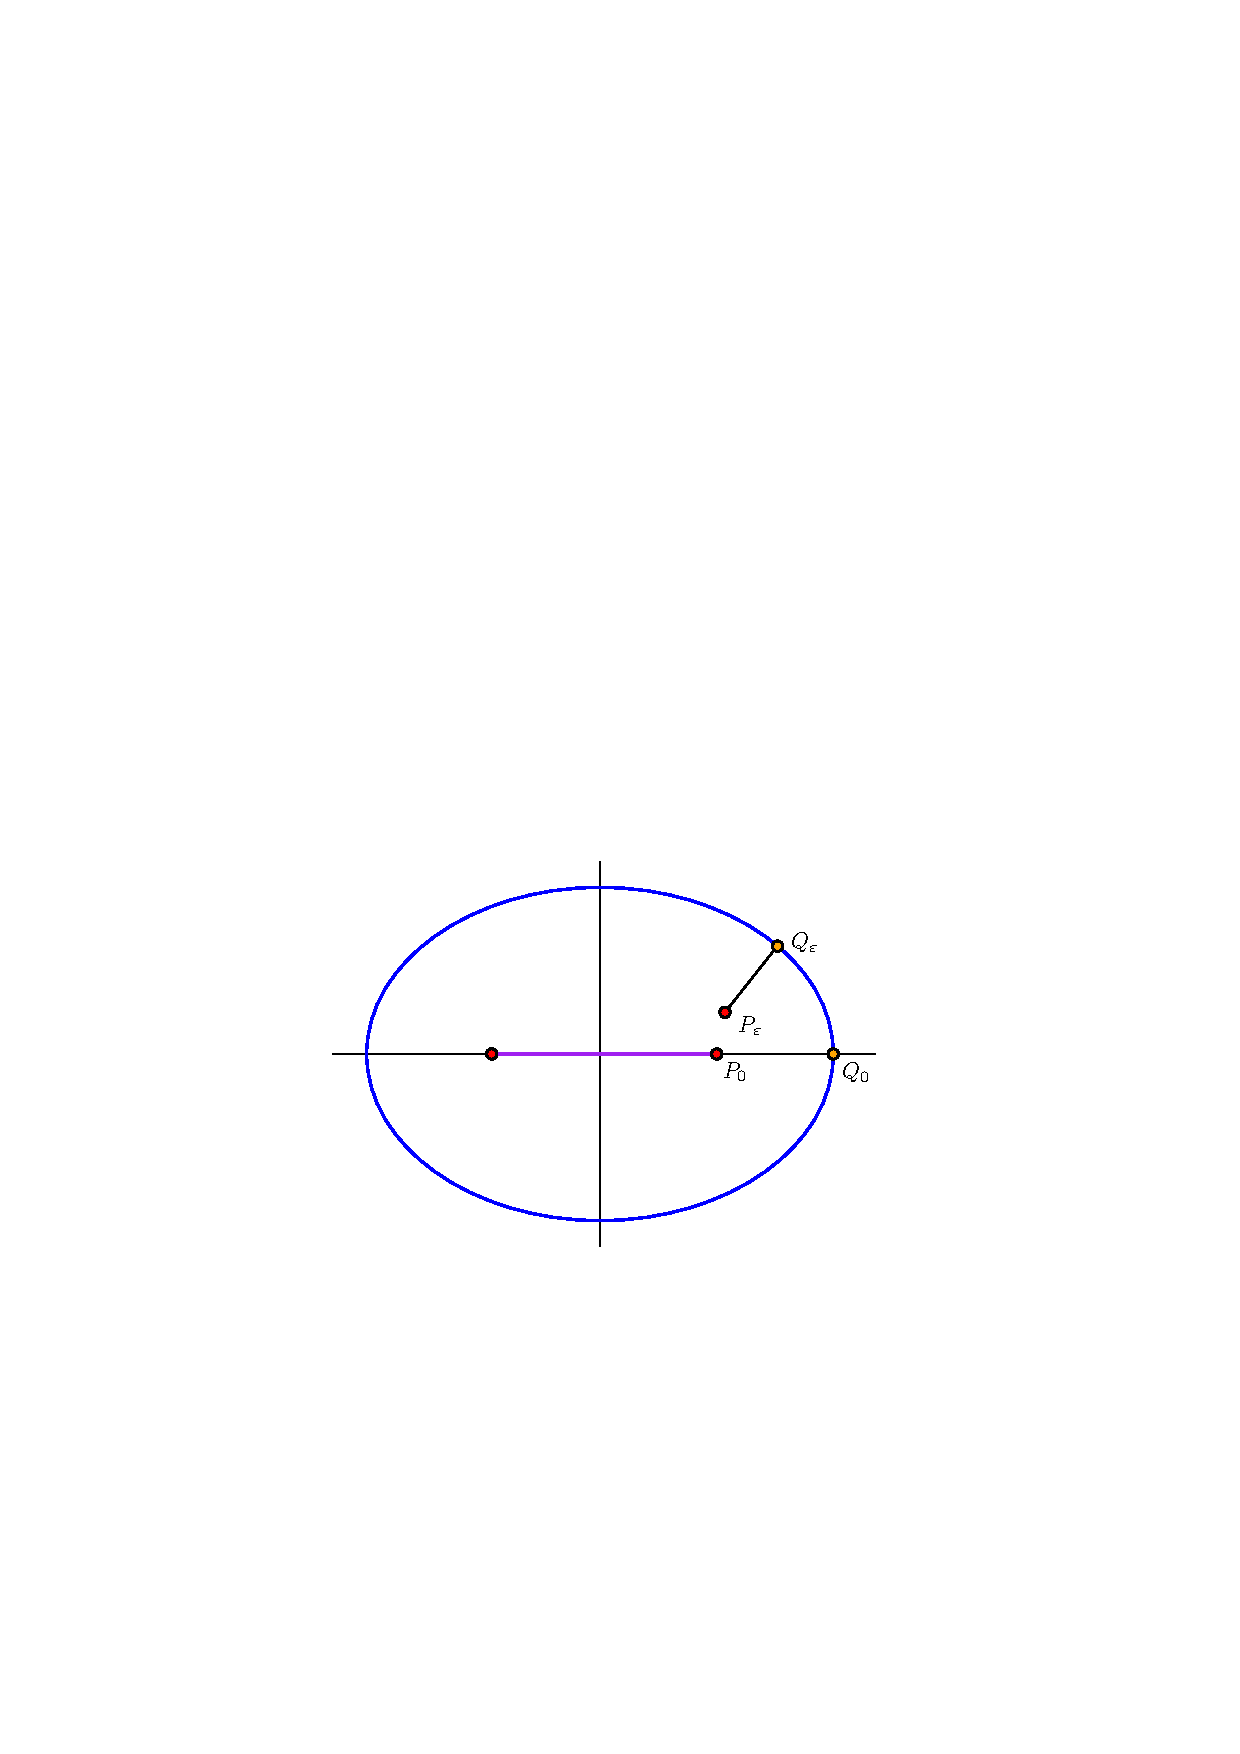
\includegraphics[scale=0.7]{Ellipse_cut.pdf}
        \caption{Cut locus of an ellipse}
    \end{figure}
    \begin{displaymath}
        x_\ep=\frac{a^2(\frac{a^2-b^2}{a}+\ep\alpha)}{t+a^2},\,\,y_\ep=\frac{b^2 \ep\beta}{t+b^2}.
    \end{displaymath}
    It follows that
    \begin{equation}
        d_\ep^2(\alpha,\beta):=d^2(P_\ep,Q_\ep)=\frac{t^2}{a^2}\left(\frac{a^2-b^2+a\ep\alpha}{t+a^2}\right)^2+\frac{t^2}{b^2}\left(\frac{b\ep\beta}{t+b^2}\right)^2\label{dsqellip}
    \end{equation}
    Using $t(0)=-b^2$ and simplifications lead us to the following
\begin{align*}
    \lim_{\ep\to 0^+}\frac{d_\ep^2-d_0^2}{\ep} & =\frac{2ab^4\alpha}{a^2(a^2-b^2)}-\lim_{\ep\to 0^+}\left(\frac{(t+b^2)(a^2b^2-a^2 t+2b^2t)}{\ep(t+a^2)^2}-\beta^2 \frac{t^2\ep}{(t+b^2)^2}\right)\\
    & = \frac{2ab^4\alpha}{a^2(a^2-b^2)}-\frac{2b^2}{a^2-b^2}\lim_{\ep\to 0}\frac{t+b^2}{\ep}+\beta^2 b^4\lim_{\ep\to 0}\frac{\ep}{(t+b^2)^2}\\
    & = \frac{2ab^4\alpha}{a^2(a^2-b^2)}-\frac{2ab^2\alpha}{a^2-b^2}=-\frac{2b^2\alpha}{a}.
\end{align*}
    
\hf On the other hand, for $\ep<0$, the point $P_\ep(\alpha,\beta)$ lies in the fourth quadrant. By symmetry, the distance between $P_\ep(\alpha,\beta)$ and $Q_\ep(\alpha,\beta)$ is the same as that between $P_{-\ep}(-\alpha,\beta)$ and $Q_{-\ep}(-\alpha,\beta)$. However, it is seen that 
    \begin{displaymath}
        d^2(P_{-\ep}(-\alpha,\beta), Q_{-\ep}(-\alpha,\beta))=d^2_{-\ep}(-\alpha,\beta)
    \end{displaymath}
    as defined in \eqref{dsqellip}. Therefore,
    \begin{align*}
        \lim_{\ep\to 0^-}\frac{d^2(P_{\ep}(\alpha,\beta), Q_{\ep}(\alpha,\beta))-d^2(P_{0}(\alpha,\beta), Q_{0}(\alpha,\beta))}{\ep} & =  \lim_{\ep\to 0^-}\frac{d^2 _{-\ep}(-\alpha,\beta)-d^2 _0(-\alpha,\beta)}{\ep}\\
        & =  -\lim_{-\ep\to 0^+}\frac{d^2 _{-\ep}(-\alpha,\beta)-d^2 _0(-\alpha,\beta)}{-\ep}\\
        & = -\frac{2b^2\alpha}{a},
    \end{align*}
    where the last equality follows from the right hand derivative of $d^2$, as computed previously.
    
    \vspace{0.1cm}
    \hf When $\beta=0$ we would like to compute $d^2_\ep(\alpha,0)$. If $\ep>0$, then 
    \begin{equation}
        \label{dsqP01}d^2_\ep(\alpha,0)=(b^2/a-\ep\alpha)^2=\frac{b^4}{a^2}-\frac{2b^2\alpha\ep}{a}+\alpha^2\ep^2.
    \end{equation}
    On the other hand, if $\ep<0$ is sufficiently small, then there are two points on the ellipse closest to $P_\ep(\alpha,0)=(\frac{a^2-b^2}{a}+\ep\alpha,0)$, with exactly one on the first quadrant, say $Q_\ep$. Since the segment $P_\ep Q_\ep$ must be orthogonal to the tangent to the ellipse at $Q_\ep$, we obtain the coordinates for $Q_\ep$:
    \begin{displaymath}
        x_\ep=\frac{a^2(\frac{a^2-b^2}{a}+\ep\alpha)}{a^2-b^2},\,\,y^2_\ep=b^2\bigg(1-\frac{x_\ep^2}{a^2}\bigg),\,\,y_\ep>0.
    \end{displaymath}
    We may compute the distance
    \begin{equation}
        \label{dsqP02}d^2_{\ep}(\alpha,0):=(d(P_\ep,Q_\ep))^2=\frac{b^4}{a^2}-\frac{2b^2\alpha\ep}{a}-\frac{b^2\alpha^2\ep^2}{a^2-b^2},
    \end{equation}
    where $\ep<0$. Combining \eqref{dsqP01} and \eqref{dsqP02} we conclude that $d^2$ is differentiable at $P_0=(\frac{a^2-b^2}{a},0)$, a point in $\cutn$ but not in $\sen$. However, comparing the quadratic part of $d^2$ in \eqref{dsqP01},\eqref{dsqP02} we conclude that $d^2$ is not twice differentiable at $P_0$. 
\end{eg}

\section{Characterizations of \texorpdfstring{\cutn}{Cu(N)}}\label{sec:characterizationOfCutLocus}
\hfb Let $(M,g)$ be a complete Riemannian manifold with distance function $d$. The exponential map \index{exponential map} at $p\in M$
\begin{displaymath}
    \exp_p:T_p M \to M
\end{displaymath}
is defined on the tangent space of $M$. Moreover, there exists minimal geodesic joining any two points in $M$. However, not all geodesics are distance realizing. Given $v\in T_p M$ with $\|v\|=1$, let $\gamma_v$ be the geodesic initialized at $p$ with velocity $v$. Let $S(TM)$ denote the unit tangent bundle and let $ [0,\infty]$ be the one point compactification of $ [0,\infty)$. Define 
\begin{displaymath}
    s:S(TM)\to [0,\infty],\,\,s(v):=\sup\{t\in [0,\infty)\,|\,\gamma_v |_{[0,t]}\,\,\textup{is minimal}\}.
\end{displaymath}

\begin{defn}[Cut Locus]\label{cutlocus2}
    Let $M$ be a complete, connected Riemannian manifold. If $s(v)<\infty$ for some $v\in S(T_pM)$, then $\textup{exp}_p(s(v)v)$ is called a \textit{cut point}. The collection of cut points is defined to be the cut locus of $p$.
\end{defn}

\vspace{0.3cm}
\hf As geodesics are locally distance realizing, $s(v)> 0$ for any $v\in S(TM)$. The following result \cite[Proposition 4.1]{Sak96} will be important for the underlying ideas in its proof.
\begin{prop}\label{scts}
    The  map $s:S(TM)\to [0,\infty], u\mapsto s(u)$ is continuous.
\end{prop}
\vspace{0.3cm}
\noindent The proof relies on a characterization of $s(v)$ provided $s(v)<\infty$, (\Cref{thm:CharacterizationOfCutLocusInTermsOfConjugatePoint}). A positive real number $T$ is $s(v)$ if and only if $\gamma_v:[0,T]$ is minimal and at least one of the following holds:\\
\hf (i) $\gamma_v(T)$ is the first conjugate point of $p$ along $\gamma_v$,\\
\hf (ii) there exists $u\in S(T_pM), u\neq v$ such that $\gamma_u(T)=\gamma_v(T)$.

\begin{rem}
    If $M$ is compact, then it has bounded diameter, which implies that $s(v)<\infty$ for any $v\in S(TM)$. The converse is also true: if $M$ is complete and connected with $s(v)<\infty$ for any $v\in S(TM)$, then $M$ has bounded diameter, whence it is compact. 
\end{rem}

\subsection{Characterization in terms of focal points}
\hfb We shall be concerned with closed Riemannian manifolds in what follows. Let $N$ be an embedded submanifold inside a 
closed, i.e., compact without boundary, manifold $M$. Let $\nu$ denote the normal bundle of $N$ in $M$ with $D(\nu)$ denoting the unit disk bundle. In the context of $S(\nu)$, the unit normal bundle and the cut locus of $N$, distance minimal geodesics or $N$-geodesics are relevant (see \Cref{distmin,cutlocus1}). We want to consider 
\begin{equation}\label{snu}
    \rho:S(\nu)\to [0,\infty),\,\,\rho(v):=\sup\{t\in [0,\infty)\,|\,\gamma_v |_{[0,t]}\,\,\textup{is an $N$-geodesic}\}.
\end{equation}
Notice that $0<\rho(v)\leq s(v)$ for any $v\in S(\nu)$. In the special case when $N=\{p\}$, $\rho$ is simply the restriction of $s$ to $T_p M$. The continuity of $\rho$ requires a result similar to \Cref{thm:CharacterizationOfCutLocusInTermsOfConjugatePoint}, which requires the definition of focal points.  
\begin{defn}[Focal point]\index{focal point}\label{defn:focalPoint}
    Let $p\in N$ and $(p,v)\in S(\nu)$. We say that $v$ is a \emph{tangent focal point}\index{tangent focal point} of $N$ if $d (\exp_\nu)_v$ is not of full rank. If $\gamma$ is a geodesic from $0$ to $v$ in $\nu_p$, then $\exp_\nu(v)$ is called a \emph{focal point of $N$ along $\exp_\nu(\gamma)$}.
\end{defn}
\vspace{0.3cm}
\begin{figure}[!htb]
    \centering
    \incfig[0.5]{FocalPoints}
    \caption{Focal points\label{fig:FocalPoints}}
\end{figure}

\hf The nullity of $d\exp_\nu$ at $v$ is called the \textit{multiplicity} of a focal point.\index{muliplicity of focal point} If it is one, we say it the \textit{first focal point}.\index{first focal point}  Analogous to \Cref{thm:CharacterizationOfCutLocusInTermsOfConjugatePoint}, we have the following result.
\begin{thm}\label{thm:CharacterizationOfCutLocusInTermsOfFocalPoint}
    Let $u\in S_p(\nu)$. A positive real number $T$ is $\rho(u)$ if and only if $\gamma_u:[0,T]$ is an $N$-geodesic and at least one of the following holds:
    \begin{enumerate}[(i)]
        \item $\gamma_u(T)$ is the first focal point of $N$ along $\gamma_u$,
        \item there exists $v\in S(\nu)$ with $v\neq u$ such that $\gamma_v(T)=\gamma_u(T)$.
    \end{enumerate}
\end{thm}

\vspace{0.3cm}
\noindent In order to prove the above theorem, we need the following observations.

\vspace{0.3cm}
\noindent \textbf{Observation A}\,\textup{\cite[Lemma 2.11, page 96]{Sak96}}\,\,\textit{Let $N$ be a submanifold of a Riemannian manifold $M$ and $\gamma:[t_0,\infty)\to M$ a geodesic emanating perpendicularly from $N$. If $\gamma(t_1)$ is the first focal point of $N$ along $\gamma$, then for $t>t_1$, $\gamma|_{[t_0,t_1]}$ cannot be an $N$-geodesic, i.e., $L\paran{\gamma|_{[t_0,t]}}>d(N,\gamma(t))$.}\\[0.2cm]
\noindent Recall that a sequence $\{\gamma_n\}$ of geodesics, defined on closed intervals, is said to converge to a geodesic $\gamma$ if $\gamma_{n}(0)\to \gamma(0)$ and $\gamma_n'(0)\to \gamma'(0)$. It follows from the continuity of the exponential map that if $t_n\to t$, then $\gamma_n(t_n)\to \gamma(t)$.\\[0.3cm]
\textbf{Observation B}\,\,\textit{Let $\gamma_n$ be a sequence of unit speed $N$-geodesics joining $p_n=\gamma_n(0)$ to $q_n=\gamma_n(t_n)$. If $\gamma_n$ converges to a geodesic $\gamma$ and $t_n\to l$, then $\gamma$ is a unit speed $N$-geodesic joining $p=\lim_n p_n$ to $q \defeq \gamma(l)=\lim_n \gamma_n(t_n)$.}
\begin{proof}
    The unit normal bundle $S(\nu)$ is closed. Since $\gamma_n'(0)\to \gamma'(0)$, it follows that $\gamma'(0)\in S(\nu)$. Note that
        \begin{displaymath}
        d(N,q) = \lim_{n\to \infty} d(N,q_n) = \lim_{n\to \infty} d(p_n,q_n)= \lim_{n\to \infty} t_n = l = L\paran{\gamma|_{[0,l]}}
        \end{displaymath}
    implies that $\gamma$ is an $N$-geodesic.
\end{proof}

\begin{proof}[Proof of \Cref{thm:CharacterizationOfCutLocusInTermsOfFocalPoint}]
    If $\gamma_u(t)$ is the first focal point of $N$ along $\gamma_u$, then Observation A implies that $\gamma_u$ cannot be minimal beyond this value. If (ii) holds, then we need to show that for sufficiently small $\varepsilon>0~$ $\gamma_u|_{[0,T+\varepsilon]}$ is not minimal. Suppose, on the contrary, that $\gamma_u$ is minimal beyond $T$. Take a minimal geodesic $\beta$ joining $\gamma_{v}(T-\varepsilon)$ to $\gamma_{u}(T+\varepsilon)$. Observe that,
	\begin{align*}
	    2\varepsilon & = d\paran{\gamma_{u}(T+\varepsilon),\gamma_u(T)} + d\paran{\gamma_v(T),\gamma_v(T-\varepsilon)} \\
        & > d\paran{\gamma_u(T+\varepsilon),\gamma_v(T-\varepsilon)}.
	\end{align*}
    If $p,q,r\in M$ such that $d(p,q)+d(q,r) = d(p,r)$ and there exist the shortest normal geodesic $\gamma_{1}$ and $\gamma_{2}$ joining $p$ to $q$ and $q$ to $r$, respectively, then $\gamma_{1}\cup \gamma_2$ is smooth at $q$ and defines a shortest normal geodesic joining $p$ to $r$. Therefore, we have
    \begin{align*}
		L(\gamma_v|_{[0,T-\varepsilon]}\cup \beta) & = T-\varepsilon + d(\gamma_v(T-\varepsilon),\gamma_u(T+\varepsilon)) \\
        & < T + \varepsilon = L(\gamma_u|_{[0,T+\varepsilon]}).
	\end{align*}
    This contradiction establishes that $\gamma_u|_{[0,T+\varepsilon]}$ is not minimal.
    
    \vspace{0.1cm}
    \hf For the converse, set $T=\rho(u)$ and observe that $\gamma_u|_{[0,T]}$ is an $N$-geodesic. Assuming that $q\defeq \gamma_{u}(T)$ is not the first focal point of $N$ along $\gamma_{u}$, we will prove that (ii) holds. Let $p=\gamma_u(0)$ and choose a neighbourhood $\tilde{U}$ of $Tu$ in $\nu$ such that $\exp_{\nu}|_{\tilde{U}}$ is a diffeomorphism. For sufficiently large $n$, $q_{n}\defeq \gamma_{u}\paran{T+1/n}\in \exp_{\nu}(\tilde{U})$. Take $N$-geodesics $\gamma_{n}$ parametrized by arc-length joining $p_n$ to $q_{n}$ and set $u_{n}\defeq \dot{\gamma}_{n}(0)\in S((T_{p_n}N)^\perp)$. Since $S((T_{p_n}N)^\perp)$ is compact, by passing to a subsequence, we may assume that $u_{n}$ converges to $v\in S(N_{p})$. By Observation B, 
	\begin{displaymath}
	    \gamma_v(T) = \lim_{n\to \infty} \gamma_{u_n}\paran{T+\textstyle{\frac{1}{n}}} = \gamma_u(T).
	\end{displaymath}
    If $v = u$, then for sufficiently large $n$, $d(p,q_n)u_{n} \in \tilde{U}$, whence 
	\begin{displaymath}
	    \paran{T+\textstyle{\frac{1}{n}}}u = d(p,q_n)u_n.
	\end{displaymath}
    Taking absolute values on both sides imply $T+1/n>d(p,q_n)$. This contradiction implies $v\neq u$.
\end{proof}
\hf We now will prove that the map $\rho$ defined in \ref{snu} is a continuous function.
\begin{prop}\label{snucts}
    The map $\rho:S(\nu)\to [0,\infty)$, as defined in \eqref{snu}, is continuous.
\end{prop}
\begin{proof}
    We will prove that $\rho(u_n)\to \rho(u)$ whenever $(p_n,u_n)\to (p,u)$ in the unit normal bundle $S(\nu)$. Let $T$ be any accumulation point of the sequence $\{\rho(u_n)\}$ including $\infty$. By Observation B, $\gamma_{u}|_{[0,T]}$ is an $N$-geodesic and hence $T\le \rho(u)$. If $T=+\infty$, we are done. So let us assume that $T<+\infty$. From \Cref{thm:CharacterizationOfCutLocusInTermsOfFocalPoint}, at least one of the following holds for infinitely many $n$.
    \begin{enumerate}[(i)]
        \item The sequence $\rho(u_n)$ is the first focal point to $N$ along $\gamma_{u_n}$
        \item  there exist $v_{n}\in S(\nu)$,  $v_{n}\neq u_n$ with $\gamma_{u_n}\paran{\rho(u_n)} = \gamma_{v_n}\paran{\rho(u_n)}$.
    \end{enumerate}

    \hf If (i) is true for infinitely many $n$, then choose infinitely many unit vectors $\{w_n\}$ which belong to the kernel $\ker \paran{D\exp_{\nu}(\rho(u_n)u_n)}$ and are contained in a compact subset of $S(\nu)$. Choose a convergent subsequence whose limit $w$ is contained in $\ker \paran{D\exp_{\nu}{(Tu)}}$. Since $w\neq 0$, the rank of $D\exp_{\nu}{(Tu)}$ is less than $\dim M$. Thus, $\gamma_{u}(T)$ is the first focal point of $N$ along $\gamma_u$ and $T=\rho(u)$.

    \vspace{0.1cm}
    \hf If (ii) is true for infinitely many $n$, then we may assume that $v_{n}\to v\in S(\nu)$. If $v\neq u$, then \Cref{thm:CharacterizationOfCutLocusInTermsOfFocalPoint} (ii) holds for $T$, whence $T=\rho(u)$. If $v=u$, we claim that $\gamma_{u}(T)$ is the first focal point of $N$ along $\gamma_{u}$. If not, then the map $\exp_{\nu}$ is regular at $Tu\in \nu$ and hence the map 
    \begin{displaymath}
        \Phi:\nu\to M\times M,~(p,u)\mapsto (p,\exp_\nu(p,u))
    \end{displaymath}
    is regular at $Tu$. Therefore, $\Phi$ is a diffeomorphism if restricted to an open neighbourhood $\tilde{U}$ of $Tu$ in $\nu$. Since $v=u$, which implies for sufficiently large $n$,~ $(p_n,\rho(u_n)u_n)$ and $(p_n,\rho(u_n)v_n)$ belong to $\tilde{U}$ and are different. On the other hand, by assumption $\Phi(\rho(u_n)u_n) = \Phi(\rho(u_n)v_n) $, which is a contradiction. Therefore, $\gamma_u(T)$ is the first focal point and $T=\rho(u)$. 
\end{proof}

\subsection{Characterization in terms of separating set}
\hfb Recall that the separating set \index{separating set} of $N$, $\sen$, consists of all points $q\in M$ such that at least two distance minimal geodesics from $N$ to $q$ exist. If $q\in \sen$ but $q\not\in \cutn$, then we have \Cref{fig: notDifferentiable}, i.e., $\gamma_1$ is an $N$-geodesic beyond $q$ while $\gamma_2$ is another $N$-geodesic for $q$. The triangle inequality applied to $\gamma_1(0)$, $q=\gamma_1(l)$ and $\gamma_2(l+\tau)$ implies that 
\begin{displaymath}
    d(\gamma_2(l+\tau),N)< l+\tau
\end{displaymath}
while for $\tau$ small enough $d(\gamma_2(l+\tau),N)=l+\tau$ as $\gamma_2$ is an $N$-geodesic beyond $q$. This contradiction establishes the well-known fact $\sen\subseteq \cutn$. In quite a few examples, these two sets are equal (see \Cref{eg:CutLocusOfEllipse} where these two are not same). In the case of $M=\mathbb{S}^n$ with $N=\{p\}$, the set $\sen$ consists of $-p$. There is an infinite family of minimal geodesics joining $p$ to $-p$. An appropriate choice of a pair of such minimal geodesics would create a loop, which is permissible in the definition of $\sen$. According to \Cref{thm:CharacterizationOfCutLocusInTermsOfFocalPoint}, a cut point is either a first focal point of $N$ along a geodesic or it is a separating point. We will now prove our one of the observations in the last chapter, that  cut locus of a submanifold $N$ is the closure of separating set of $N$. 
\begin{thm}\label{thm: Theorem 2}\label{thm:SeClosureIsCutLocus}
    Let $\cutn$ be the cut locus of a compact submanifold $N$  of a  complete Riemannian manifold $M$. The subset $\sen$ of $\cutn$ is dense in $\cutn.$
\end{thm}
\begin{proof}
    Let $q\in \cutn $ but not in $\sen$. Choose an $N$-geodesic $\gamma$ joining $N$ to $q$ such that any extension of $\gamma$ is not an $N$-geodesic. This geodesic $\gamma$ is unique as $q\notin \sen$. We may write $\gamma(t) = \exp_\nu(tx)$, where $\gamma(0)=p\in N$ and $\gamma'(0)=x_0\in S(\nu_p)$. It follows from the definition of $\rho$ that $q=\exp_\nu\paran{\rho(x_0)x_0}$. We need to show that every neighborhood of $q$ in $\cutn$ must intersect $\sen$. Suppose it is false. Let $\delta>0$ and consider $\Ball$, the closed ball with center $x_0$ and radius $\delta$. Define the cone
    \begin{equation*}
        \co\! \defeq \curlybracket{tx:0\le t\le 1,~ x\in \Ball\cap S(\nu)}.
    \end{equation*}
    Since $\Ball\cap S(\nu)$ is homeomorphic to a closed $(n-1)$-ball for sufficiently small $\delta$, the cone will be homeomorphic to a closed Euclidean $n$-ball.
    \begin{figure}[H] 
        \centering 
        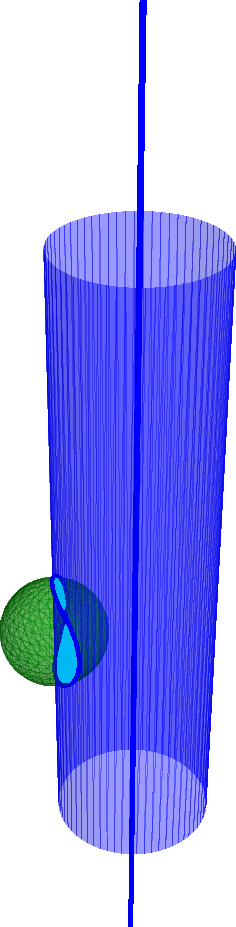
\includegraphics[angle=270, scale=0.8]{Cone1.pdf} 
        \caption{\co} 
        \label{fig: cone} 
    \end{figure}
    \noindent Similarly, define another cone
    \begin{equation*}
        \costar\! \defeq \big\{\rho\paran{ x/\norm{x}}x\,|\, x\in \co\!, ~x\neq 0\big\}\cup \{0\}.
    \end{equation*} 
    Note that $\rho(x_0)$ is finite. As $\rho$ is continuous, due to \Cref{snucts}, for sufficiently small $\delta$ the term $\rho\paran{x/\norm{x}}$ is still finite, whence \costar is well defined. We claim that \costar is also homeomorphic to a closed Euclidean $(n-k)$-ball. Indeed,  a non-zero $x\in \co\!$ implies $x=\lambda \hat{x}$, for some $\lambda \in (0,1]$ and $\hat{x}\in \Ball\cap S(\nu)$. Since $\rho(\hat{x})x = \lambda \rho(\hat{x})\hat{x}$, it follows that \costar is the cone of the set
    \begin{displaymath}
        \{\rho(\hat{x})\hat{x}\,|\,\hat{x}\in \Ball\cap S(\nu)\},
    \end{displaymath}
    which is homeomorphic to $\Ball\cap S(\nu)$. Now we have a dichotomy: 
    \begin{enumerate}[(a)]
        \item For a fixed small $\delta>0$, the restriction of $\exp_\nu$ to \costar is a homeomorphism to its image because it is injective, or
        \item For any $\delta>0$, the restriction of $\exp_\nu$ to \costar is not injective.
    \end{enumerate}
    If (b) holds, choose $v_n\neq w_n\in \mathrm{Co}^\star(x_0,\frac{1}{n})$ such that these map to $q_n$ under $\exp_\nu$. Thus,  $q_n\in \sen$ and compactness of $S(\nu)$ ensures that $q_n$ converges to $q$. If (a) holds, then let $B(q,\varepsilon)$ denote the open ball in $M$ centered at $q$ with radius $\varepsilon>0$. We claim that it intersects the complement of $\exp_\nu(\costar\!\!)$ in $M$. But it is true as $\rho(x_0)x_0$ lies on the boundary of \costar and hence it has a neighborhood in \costar which is homeomorphic to a closed $n$-dimensional Euclidean half plane. Since $\exp_{\nu}$ restricted to \costar was a homeomorphism, the open ball $B(q,\varepsilon)$ must intersect the points outside the image of $\exp_{\nu}(\costar\!\!)$. 

    \vspace{0.2cm}
    \hf Now take $\varepsilon = \frac{1}{n}$. For each $n$, there exists $q_{n}\in B\paran{q,\frac{1}{n}}$ such that $q_{n}\notin \exp_{\nu}(\costar\!\!)$. Since $M$ is complete, for each point $q_{n}$ let $\gamma_{n}$ be a $N$-geodesics joining $p_n\in N$ to $q_{n}$. We may invoke the following result from Buseman's book \cite[Theorem 5.16, page 24]{Bus55}. Let $\curlybracket{\gamma_{n}}$ be a sequence of rectifiable curves in a finitely compact set $X$ and the lengths $\ell(\gamma_n)$ are bounded. If the initial points $p_{n}$ of $\gamma_{n}$ forms a bounded set, then $\curlybracket{\gamma_n}$ contains a subsequence $\gamma_{n_k}$ which converges uniformly to a rectifiable curve $\tilde{\gamma}$ in $X$ and 
    \begin{equation*}\label{Fact A eqn: 1} 
        \ell(\tilde{\gamma}) \le \lim\inf \ell\paran{\gamma_{n_k}}
    \end{equation*}
    Since $\{p_n\}$ lie in the compact set $N$, we obtain a rectifiable curve $\tilde{\gamma}$ such that 
    \begin{displaymath}
        \ell(\tilde{\gamma})\leq  \lim\inf \ell\paran{\gamma_{n_k}}=\lim_k \ell(\gamma_{n_k})=\lim_k d(q_{n_k},N)=d(q,N).
    \end{displaymath}
    Thus, $\tilde{\gamma}$ is actually an $N$-geodesic joining $p'=\lim_k p_{n_k}$ to $q$  and the unit tangent vectors $x_{n_k}=\gamma_{n_k}'(0)$ at $p_{n_k}$ converges to the unit tangent vector $\tilde{x}=\tilde{\gamma}'(0)$ at $p'$.  Since $x_{0}$ is an interior point of the set $\Ball\cap S(\nu)$, any sequence in $S(\nu)$ converging to $x_{0}$ must eventually lie in \co\!. According to our choice, $q_{n_k}\notin \exp_{\nu}(\costar\!\!)$ and $x_{n_k}$ all lie outside of \co\!. Hence $x_{0}\neq \tilde{x}$ and $\gamma \neq \tilde{\gamma}$. Thus, there are two distinct $N$-geodesics $\gamma$ and $\tilde{\gamma}$ joining $N$ to $q$, a contradiction to $q\notin \sen$. This completes the proof.
\end{proof}

\section{Topological properties}\label{sec:topologicalProperties}
\hfb In this section we will study the structure of the cut locus and the relation of cut locus to the Thom space. We will also see various applications of this relation.
\subsection{Structure of the cut locus}
\hfb On a complete Riemannian manifold it is very difficult to analyze the structure of cut locus of a point or a submanifold. The main problem is that cut locus is not $C^1$-smooth\index{$C^1$-smooth}. For example, the authors in \cite{GlSi78} showed that cut locus of a point is not always triangulable\index{triangulable}. Regarding the question of cut loci being triangulable, we recall the result \cite{Buc77} that the cut locus (of a point) of a real analytic Riemannian manifold (of dimension $d$) is a simplicial complex of dimension at most $d-1$. It follows, without much changes, that the result holds for cut loci of submanifolds as well. Hence, we attribute the following result to Buchner. 

\begin{thm}[Buchner 1977]\label{Buchner}
    Let $N$ be an analytic submanifold of a real analytic manifold $M$. If $M$ is of dimension $d$, then the cut locus $\cutn$ is a simplicial complex of dimension at most $d-1$.
\end{thm}
\vspace{0.3cm}
\noindent The obvious modifications to the proof by Buchner are the following:
\begin{enumerate}[(i)]
    \item Choose $\ep$ to be such that there is a unique geodesic from $p$ to $q$ if $d(p,q)<\ep$ and if $d(N,q)<\ep$, then there is a unique $N$-geodesic to $q$;
    \item  Consider the set $\Omega_N(t_0,t_1,\ldots,t_k)$, the space of piecewise broken geodesics starting at $N$, and define $\Omega_N(t_0,t_1,\ldots,t_k)^s$ analogously;
    \item The map
    \begin{displaymath}
        \Omega_N(t_0,t_1,\ldots,t_k)^s\to N\times M\times \cdots\times M,\,\,\omega\mapsto (\omega(t_0),\omega(t_1),\ldots,\omega(t_k))
    \end{displaymath}
    determines an analytic structure on $\Omega_N(t_0,t_1,\ldots,t_k)^s$.
\end{enumerate}
The remainder of the proof works essentially verbatim.

\begin{rem}
    As we have seen in \Cref{join}, the dimension of the cut locus of a $k$-dimensional submanifold can be of dimension $d-k-1$. However, generically, we may not expect this to be true. In fact, for real analytic knots (except the unknot) in $\mathbb{S}^3$, it is always the case that the cut locus cannot be homotopic to a (connected) $1$-dimensional simplicial complex (cf \Cref{codim2}). 
\end{rem}

\subsection{Thom space via cut locus}\label{Sec: Thom}
\hfb Recall that the \textit{Thom space} \index{Thom space} $\textup{Th}(E)$ of a real vector bundle \index{vector bundle} $E\to B$ of rank $k$ is $D(E)/S(E)$, where it is understood that we have chosen a Euclidean metric on $E$. If $B$ is compact, then the Thom space $\textup{Th}(E)$ is the one-point compactification \index{one-point compactification} of $E$. In general, we compactify the fibres and then collapse the section at infinity to a point to obtain $\textup{Th}(E)$. Thus, Thom spaces obtained via two different metrics are homeomorphic. We start with a similar exponential map which is obtained by the $\rho$ map, and we named it \textit{rescaled exponential map}. \index{rescaled exponential map}  

\begin{defn}[Rescaled Exponential]\index{rescaled exponential map}
    The \textit{rescaled exponential} or $\rho$-exponential map is defined to be 
    \begin{displaymath}
        \widetilde{\textup{exp}}:D(\nu)\to M,\,\,(p,v)\mapsto \left\{
        \begin{array}{rl}
            \textup{exp}_p(\rho(\hat{v})v) & \textup{if $v=\|v\|\hat{v}\neq 0$}\\
            p & \textup{if $v=0$.}
        \end{array}\right.
    \end{displaymath}
\end{defn}

\vspace{0.3cm}
\noindent We are now ready to prove the main result of this section.

\begin{thm}\label{Thomsp}
    Let $N$ be an embedded submanifold inside a closed, connected Riemannian manifold $M$. If $\nu$ denotes the normal bundle\index{normal bundle} of $N$ in $M$, then there is a homeomorphism 
    \begin{displaymath}
        \widetilde{\textup{exp}}:D(\nu)/S(\nu)\stackrel{\cong}{\longrightarrow} M/\cutn.
    \end{displaymath}
\end{thm}
\begin{proof}
    It follows from \Cref{snucts} that the rescaled exponential is continuous. Moreover, $\widetilde{\textup{exp}}$ is surjective and $\widetilde{\textup{exp}}(S(\nu))=\cutn$. If there exists $(p,v)\neq (q,w)\in D(\nu)$ such that 
    \begin{displaymath}
        \widetilde{\textup{exp}}(p,v)=\widetilde{\textup{exp}}(q,w)=p',
    \end{displaymath}
    then $d(p',N)$ can be computed in two ways to obtain 
    \begin{displaymath}
        d(p',N)=\rho(\hat{v})\|v\|=\rho(\hat{w})\|w\|.
    \end{displaymath}
    Thus, $T=d(p',N)$ is a number such that $\gamma_v:[0,T]$ is an $N$-geodesic and $\gamma_v(T)=\gamma_w(T)=p'$. By \Cref{thm:CharacterizationOfCutLocusInTermsOfFocalPoint}, we conclude that $T=\rho(\hat{v})=\rho(\hat{w})$, whence $\|v\|=\|w\|=1$. Therefore, $\widetilde{\textup{exp}}$ is injective on the interior of $D(\nu)$. \\
    \hfb As $\cutn$ is closed and $M$ is a compact metric space, the quotient space $M/\cutn$ is Hausdorff. As the quotient $D(\nu)/S(\nu)$ is compact, standard topological arguments imply the map induced by the rescaled exponential is a homeomorphism.
\end{proof}

\vspace{0.3cm}
\hf We will now revisit a basic property of Thom space via its connection to the cut locus. It can be seen that 
\begin{equation}\label{cutprod}
    \mathrm{Cu}(N_1\times N_2)=(\mathrm{Cu}(N_1)\times M_2)\cup (M_1\times \mathrm{Cu}(N_2))
\end{equation}
for an embedding $N_1\times N_2$ inside $M_1\times M_2$. If $\nu_j$ is the normal bundle of $N_j$ inside $M_j$, then \Cref{Thomsp} along with \eqref{cutprod} implies that
\begin{align*}
    \textup{Th}(\nu_1\oplus \nu_2) & \cong \frac{M_1\times M_2}{(M_1\times \mathrm{Cu}(N_2))\cup (\mathrm{Cu}(N_1)\times M_2)}
    \\[1ex]
    & \cong \frac{M_1/\mathrm{Cu}(N_1)\times M_2/\mathrm{Cu}(N_2)}{M_1/\mathrm{Cu}(N_1)\vee M_2/\mathrm{Cu}(N_2)}
    \\[1ex]
    & \cong \textup{Th}(\nu_1)\wedge \textup{Th}(\nu_2).
\end{align*}
Let $N=N_1\sqcup N_2$ be a disjoint union of connected manifolds of the same dimension. If $N\hookrightarrow M$, then let $\nu_j$ denote the normal bundle of $N_j$ in $M$. If $\nu$ is the normal bundle of $N$ in $M$, then 
\begin{equation}\label{Thomwedge}
    \textup{Th}(\nu)\cong \textup{Th}(\nu_1)\vee \textup{Th}(\nu_2).
\end{equation}
This implies that
\begin{displaymath}
    M/\cutn \cong M/\mathrm{Cu}(N_1)\vee M/\mathrm{Cu}(N_2).
\end{displaymath}
\begin{eg}\label{eg:CutLocusOfLink}
    Consider the two circles
    \begin{displaymath}
        N_1=\{(\cos t,\sin t,0,0)\,|\,t\in\R\},\,\,N_2=\{(0,0,\cos t,\sin t)\,|\,t\in\R\}
    \end{displaymath}
    in $\mathbb{S}^3$. The link $N:=N_1\sqcup N_2$ has linking number $1$. We claim that the cut locus
    \begin{displaymath}
        \cutn=\left\{\frac{1}{\sqrt{2}}(\cos s,\sin s, \cos t,\sin t)\,|\,s,t\in\R\right\}
    \end{displaymath}
    is a torus. We will prove the claim by showing that the above set is separating set of $N$. As it is closed, the claim will follow by using \Cref{thm:SeClosureIsCutLocus}. Let $P=(a,b,0,0)\in N$ with $a^2+b^2=1$. Note that 
    \begin{displaymath}
        T_P\mathbb{S}^3 \cong T_PN\directsum \left(T_PN\right)^\perp \cong \spn\{(-b,a,0,0)\} \directsum \spn \{\mathbf{e}_3,\mathbf{e}_4\},
    \end{displaymath}  
    where $\mathbf{e}_3=(0,0,1,0)$ and $\mathbf{e}_4=(0,0,0,1)$. We take any unit vector at $P$ which is perpendicular to $T_PN$, say $\mathbf{v}=(0,0,\cos \theta, \sin \theta)$. An $N$-geodesic starting at $P$ in the direction of $\mathbf{v}$ will be
    \begin{displaymath}
        \gamma(t)=P\cos t+\mathbf{v} \sin t,~= (a\cos t,b\cos t,\cos \theta \sin t, \sin \theta \sin t),~ ~0\le t \le \pi.
    \end{displaymath} 
    We have 
    \begin{displaymath}
        d(\gamma(t),N) = \inf_{X\in N}d(\gamma(t),X) = \min\left\{\inf_{X\in N_1}d(\gamma(t),X), \inf_{X\in N_2}d(\gamma(t),X),\right\}.
    \end{displaymath}
    
    \noindent Look at \Cref{fig:DistanceFromLink} and note that 
    \begin{displaymath}
        d(X,\gamma(t)) = \cos^{-1}(X\cdot \gamma(t)).
    \end{displaymath}
    \begin{figure}[!htb]
        \centering
        \incfig[0.3]{DistanceFromLink}
        \caption{Distance of $X$ to $\gamma(t)$  \label{fig:DistanceFromLink}}
    \end{figure}
    \noindent Therefore, the problem of finding the distance of $N$ to $\gamma(t)$ is equivalent to maximizing the dot product $X\cdot \gamma(t)$.
    Let $X\in N_1$ and $X=(x,y,0,0),~x^2+y^2=1$. Then 
    \begin{displaymath}
        X\cdot \gamma(t) = ax\cos t+by\cos t.
    \end{displaymath} 
    Maximizing the above such that $x^2+y^2=1$ by the method of Lagrange multiplier, we have
    \begin{displaymath}
        x = \dfrac{a\cos t}{|\cos t|}, \text{ and } y = \dfrac{b\cos t}{|\cos t|}.
    \end{displaymath}
    Note that the above expression is well-defined, as if $\cos t =0$, then $X\cdot \gamma(t)=0$. The maximum value of $X\cdot \gamma(t)$ will be $|\cos t|$ and this is achieved by only one point of $N_1$. Similarly, if we maximize the dot product over $N_2$, we get the maximum value $|\sin t|$, which is also obtained by a single maxima. Thus, $\gamma(t)$ will be a separating point if and only if 
    \begin{displaymath}
        |\cos t| =|\sin t| \implies t = \dfrac{\pi}{4},\dfrac{3\pi}{4}.
    \end{displaymath}
    Therefore, the separating points will be
    \begin{displaymath}
        \left\{\frac{1}{\sqrt{2}}(\cos s,\sin s,\cos \theta,\sin \theta):s,\theta\in \mathbb{R}\right\}.
    \end{displaymath}
    \vspace{0.3cm}
    \hf Note that $\mathrm{Cu}(N_1)=N_2$ and vice-versa as well as 
    \begin{displaymath}
        \mathbb{S}^3/\mathrm{Cu}(N_j)\cong (S^1\times S^2)/(S^1\times \infty)
    \end{displaymath}
    where $S^1\times S^2$ is the fibrewise compatification of the normal bundle of $N_j$. We conclude that 
    \begin{displaymath}
        \mathbb{S}^3/\cutn\cong \Big(\frac{S^1\times S^2}{S^1\times \infty}\Big)\vee \Big(\frac{S^1\times S^2}{S^1\times \infty}\Big).
    \end{displaymath}
\end{eg}

\hf There are some topological similarities between $\cutn$ and $M-N$. We recall that a topological pair $(X, A)$ is called a \textit{good pair\index{good pair}} if $A$ is closed in $X$ and there is an open subset $U\subseteq X$ with $A\subseteq U$ such that $A$ is a strong deformation retract in $U$.
\begin{lemma}\label{defretM-N}
The cut locus $\cutn$ is a strong deformation retract of $M-N$. In particular, $(M,\cutn)$ is a good pair and the number of path components of $\cutn$ equals that of $M-N$.
\end{lemma}
\begin{proof}
    Consider the map $H:(M-N)\times [0,1]\to M-N$ defined via the normal exponential map 
    \begin{align*}
        H(q,t) = \begin{cases}
            \exp_\nu\left[\left\{t \cdot \rho\paran{\frac{\exp_\nu^{-1}(q) }{\norm{\exp_\nu^{-1}(q)}}}+(1-t)\norm{\exp_\nu^{-1}(q)}\right\}\frac{\exp_\nu^{-1}(q)}{\norm{\exp_\nu^{-1}(q)}}\right]  & \text{ if } q\notin \cutn \\[1ex]
            q & \text{ if } q\in \cutn.
        \end{cases}
    \end{align*}
    If $q\in M - (\cutn\cup N)$, then let $\gamma$ be the unique $N$-geodesic joining $N$ to $q$. The path $H(q,t)$ is the image of this geodesic from $q$ to the first cut point along $\gamma$. The continuity of $\rho$ implies that $H$ is continuous. It also satisfies $H(q,0)=q$ and $H(q,1)\in\cutn$. The claims about good pair and path components are clear.
\end{proof}

\begin{rem}
    The above lemma, in particular, shows that the homotopy type of the cut locus of a submanifold is independent of the choice of the Riemannian metric.
\end{rem}

\begin{cor}\label{htpy-cut-locus}
    If two embeddings $f,g:N\to M$ are ambient isotopic, then $\mathrm{Cu}(f(N))$ and $\mathrm{Cu}(g(N))$ are homotopy equivalent.
\end{cor}
\begin{proof}
    The hypothesis implies that there is a diffeomorphism $\varphi: M\to M$ such that $\varphi(f(N))=g(N)$. Thus, $M-\mathrm{Cu}(f(N))$ is homeomorphic to $M-\mathrm{Cu}(g(N))$ and the claim follows from the lemma above. Note that in the smooth category, the notion of isotopic and ambient isotopic are equivalent (refer to \S 8.1 of the book \cite{Hir76}). Thus, the same conclusion holds if we assume that the embeddings are isotopic.
\end{proof}

\begin{rem}
    Without the assumption of $M$ being closed, the above result fails to be true. One may consider $M=S^1\times \R$ with the natural product metric and $N=S^1$. In fact, the universal cover of $M$ is $\R\times \R$ while that of $N$ is $\R$. If we choose a periodic curve in $\R^2$ which is isotopic to the $x$-axis and has non-empty cut locus in $\R^2$, then we may pass via the covering map to obtain an embedding $g$ of $N$ isotopic to the embedding $f$ identifying $N$ with $S^1\times \{0\}$. For this pair, $\mathrm{Cu}(f(N))=\varnothing$ while $\mathrm{Cu}(g(N))\neq \varnothing$.
\end{rem}

\hf Several other identifications between topological invariants can be explored. For instance, if $\iota:N^k\hookrightarrow M^d$ is as before such that $M-N$ is path connected, then 
\begin{equation}\label{isopi}
    \iota_\ast:\pi_j(\cutn)\stackrel{\cong}{\longrightarrow}\pi_j(M)
\end{equation}
if $0\leq j\leq d-k-2$ while $\iota_\ast$ is a surjection for $j=d-k-1$. The proof of this relies on a general position argument, i.e., being able to find a homotopy of the sphere that avoids $N$, followed by \Cref{defretM-N}. Surjectivity of $\iota_\ast$ if $j\leq d-k-1$ is imposed by the requirement that a sphere $S^j$ in general position must not intersect $N^k$. Injectivity of $\iota$ for $j\leq d-k-2$ is imposed by the condition that a homotopy $S^j\times [0,1]$ in general position must not intersect $N^k$. This observation \eqref{isopi} generalizes a result in \cite[Proposition 4.5 (1)]{Sak96}.

\vspace{0.2cm}
\hf The inclusion $i:\cutn\hookrightarrow M$ induces a long exact sequence in homology
\begin{displaymath}
    \cdots \to H_j(\cutn)\stackrel{i_\ast}{\longrightarrow} H_j(M)\to H_j(M,\cutn)\stackrel{\partial}{\longrightarrow} H_{j-1}(\cutn)\to \cdots
\end{displaymath}
As $(M,\cutn)$ is a good pair (cf \Cref{defretM-N}), we replace the relative homology of $(M,\cutn)$ with reduced homology of $M/\cutn\cong \textup{Th}(\nu)$. This results in the following long exact sequence
\begin{equation}\label{lesThom}
    \cdots \to H_j(\cutn)\stackrel{i_\ast}{\longrightarrow} H_j(M)\stackrel{q}{\longrightarrow} \widetilde{H}_j(\textup{Th}(\nu))\stackrel{\partial}{\longrightarrow} H_{j-1}(\cutn)\to \cdots
\end{equation}
If $N=\{p\}$ is a point, then $\textup{Th}(\nu)=S^d$ and \eqref{lesThom} imply isomorphisms
\begin{displaymath}
    i_\ast:H_j(\textup{Cu}(p))\stackrel{\cong}{\longrightarrow} H_j(M),\,\,i^\ast:H^j(M)\stackrel{\cong}{\longrightarrow} H^j(\textup{Cu}(p))
\end{displaymath}
for $j\neq d,d-1$ (cf \cite[Proposition 4.5 (2)]{Sak96}). 

\begin{rem}
    The long exact sequence \eqref{lesThom} can be interpreted as the dual to the long exact sequence in cohomology of the pair $(M,N)$. If $N=N_1\sqcup \cdots\sqcup N_l$ is a disjoint union of submanifolds of dimension $k_1, \ldots, k_l$ respectively, then the Thom isomorphism implies that 
    \begin{displaymath}
        \widetilde{H}_j(\textup{Th}(\nu))\cong \widetilde{H}_j(\textup{Th}(\nu_1))\oplus \cdots\oplus \widetilde{H}_j(\textup{Th}(\nu_l))\cong H_{j-(d-k_1)}(N_1)\oplus\cdots\oplus H_{j-(d-k_l)}(N_l),
    \end{displaymath}
    where $\nu_j$ is the normal bundle of $N_j$. Applying Poincar\'{e} duality to each $N_j$, we obtain isomorphisms
    \begin{displaymath}
        \widetilde{H}_j(\textup{Th}(\nu))\cong \oplus_{i=1}^l H^{d-j}(N_i)= H^{d-j}(N).
    \end{displaymath}
    Poincar\'{e}-Lefschetz duality applied to the pair $(M,N)$ provides isomorphisms
    \begin{equation}\label{MNcutn}
        \check{H}^j(M,N)\cong H_{d-j}(M-N).
    \end{equation}
    As $M$ and $N$ are triangulable, $\check{\textup{C}}$ech cohomology may be replaced by singular cohomology. Since $M-N$ deforms to $\cutn$ by \Cref{defretM-N}, we have isomorphisms
    \begin{equation}\label{MNcutn2}
        H^j(M,N)\cong H_{d-j}(\cutn).
    \end{equation}
    Combining all these isomorphisms, we obtain the long exact sequence in cohomology for $(M,N)$ from \eqref{lesThom}. 
\end{rem}

\begin{lemma}\label{homcutn}
    Let $N$ be a closed submanifold of $M$ with $l$ components. If $M$ has dimension $d$, then $H_{d-1}(\cutn)$ is free abelian of rank $l-1$ and $H_{d-j}(\cutn)\cong H^j(M)$ if $j-2\geq k$, where $k$ is the maximum of the dimension of the components of $N$.
\end{lemma}
\begin{proof}
    It follows from \eqref{MNcutn} that 
    \begin{displaymath}
        H_{d-1}(\cutn)\cong H^1(M,N).
    \end{displaymath}
    Consider the long exact sequence associated to the pair $(M,N)$ 
    \begin{displaymath}
        0\to H^0(M,N)\to H^0(M)\stackrel{i^\ast}{\rightarrow} H^0(N)\to H^1(M,N)\to H^1(M)\to H^1(N)\to \cdots
    \end{displaymath}
    If $N$ has $l$ components, i.e., $N=N_1\sqcup \cdots\sqcup N_l$ where $N_j$ has dimension $k_j$, then $H^1(M,N)$ is torsion-free. This follows from the fact that $i^\ast(1)=(1,\ldots,1)$ and $H^1(M)$ is free abelian. 

    \vspace{0.1cm}
    \begin{rem}
        In the above  Lemma, if in particular, $H^1(M)=0$, then $H_{d-1}(\cutn)\cong \mathbb{Z}^{l-1}$.
    \end{rem}
    \hf The long exact sequence for the pair $(M,N)$ imply that there are isomorphisms
    \begin{equation}\label{cutnM}
        H_{d-j}(\cutn)\cong H^j(M,N)\stackrel{\cong}{\longrightarrow} H^j(M)
    \end{equation}
    if $j\geq k+2$, where $k=\max\{k_1,\ldots,k_l\}$. 
\end{proof}

\begin{rem}
    Cut locus can be very hard to compute. For a general space, we have the notion of topological dimension. This notion coincides with the usual notion if the space is triangulable. However, in \cite{BaMi62}, the authors proved that the singular homology of a space may be non-zero beyond its topological dimension. \v{C}ech (co)homology is better equipped to detect topological dimension and is the reason why one may prefer it over singular homology due to the generic fractal like nature of cut loci (see the remarks following \Cref{thm:ThmC} in \Cref{ch:introduction}). Although the topological dimension of $\cutn$ is at most $d-1$, it is not apparent that $H_{d-1}(\cutn)$ is a free abelian group. 
\end{rem}

\vspace{0.3cm}
\hf There are several applications of this discussion.
\begin{thm}\label{homsph}
    Let $N$ be a smooth homology $k$-sphere embedded in a Riemannian manifold homeomorphic to $S^d$. If $d\geq k+3$, then the cut locus $\cutn$ is homotopy equivalent to $S^{d-k-1}$.
\end{thm}
\begin{proof}
    As $N$ has codimension at least $3$, its complement is path-connected. It follows from \eqref{isopi} and  \Cref{defretM-N} that $M-N$ is $(d-k-2)$-connected. In particular, $M-N$ is simply-connected and by Hurewicz isomorphism, $H_j(M-N)=0$ if $j\leq d-k-2$.  Note that $H_d(M-N)=0$ as $M-N$ is a non-compact manifold of dimension $d$. 

    \vspace{0.1cm}
    \hf If $k>0$, then by  \Cref{homcutn}, $H_{d-1}(M-N)=0$. Moreover, by Poincar\'{e}-Lefschetz duality \eqref{MNcutn}, we infer that the only non-zero higher homology of $M-N$ is $H_{d-k-1}(M-N)\cong\mathbb{Z}$. By Hurewicz Theorem there is an isomorphism, $\pi_{d-k-1}(M-N)\cong\mathbb{Z}$. Let 
    \begin{displaymath}
        \alpha:S^{d-k-1}\to M - N
    \end{displaymath}
    be a generator. The map $\alpha_\ast$ induces an isomorphism on all homology groups between two simply-connected CW complexes. It follows from Whitehead's Theorem that $\alpha$ is a homotopy equivalence. Using \Cref{defretM-N}, we obtain our homotopy equivalence $H_1\comp \alpha:S^{d-k-1}\to \cutn$.

    \vspace{0.1cm}
    \hf If $k=0$, then by \Cref{homcutn}, $H_{d-1}(M-N)\cong \mathbb{Z}$. Arguments similar to the $k>0$ case now applies to obtain a homotopy equivalence with $S^{d-1}$.
\end{proof}

\hf The above result is foreshadowed by \Cref{join} where we showed that the cut locus of $N=\mathbb{S}^k_i$ inside $M=\mathbb{S}^d$ is $\mathbb{S}^{d-k-1}_l$. It also differs from Poincar\'{e}-Lefschetz duality in that we are able to detect the exact homotopy type of the cut locus. In fact, when $M$ and $N$ are real analytic and the embedding is also real analytic, then by \Cref{Buchner} we infer that $\cutn$ is a simplicial complex of dimension at most $d-1$. Towards this direction, \Cref{homsph} can be pushed further.

\begin{prop}\label{homsph2}
    Let $N$ be a real analytic homology $k$-sphere embedded in a real analytic homology $d$-sphere $M$. If $d\geq k+3$, then the cut locus $\cutn$ is a simplicial complex of dimension at most $(d-1)$, having the homology of $(d-k-1)$-sphere with fundamental group isomorphic to that of $M$.
\end{prop}

\vspace{0.3cm}
\noindent The proof of this is a combination of ideas used in the proof of \Cref{homsph}. The homotopy type cannot be deduced here due to the presence of a non-trivial fundamental group. An intriguing example can be obtained by combining \Cref{homsph2} and Poincar\'{e} homology sphere.

\begin{eg}[Cut locus of $0$-sphere in Poincar\'{e} sphere]\label{eg: Poincare}\index{ Poincar\'{e} sphere}
    Let $\tilde{I}$ be the binary icosahedral group. It is a double cover of $I$, the icosahedral group, and can be realized a subgroup of $SU(2)$. It is known that $H_1(\tilde{I};\mathbb{Z})=H_2(\tilde{I};\mathbb{Z})=0$, i.e., it is perfect and the second homology of the classifying space $B\tilde{I}$ is zero. A presentation of $\tilde{I}$ is given by
    \begin{displaymath}
        \tilde{I}=\langle s,t\,|\,(st)^2=s^3=t^5\rangle.
    \end{displaymath}
    In fact, if we construct a cell complex $X$ of dimension $2$ using the presentation above, then $X$ has one $0$-cell, two $1$-cells and two $2$-cells. The cellular chain complex, as computed from the presentation, is given by
    \begin{equation*}
        \xymatrix@R+1pc@C+2pc{
        0\ar[r] & \mathbb{Z}^2\ar[r]^{\spmat{-1 & 2 \\ 3 & -5}} & \mathbb{Z}^2\ar[r]^-{0} & \mathbb{Z}\ar[r] & 0
        }
    \end{equation*}
    Therefore, $H_1(X)=H_2(X)=0$ while $\pi_1(X)=\tilde{I}$. 

    \hf In contrast, consider the cut locus $C$ of the $0$-sphere in $SU(2)/\tilde{I}$, the Poincar\'{e} homology sphere. As $SU(2)$ is real analytic, so is the homology sphere. By \Cref{homsph2}, $C$ is a finite, connected simplicial complex of dimension $2$ such that $\pi_1(C)\cong \tilde{I}$ and $H_\bullet(C;\mathbb{Z})\cong H_\bullet(S^2;\mathbb{Z})$. The existence of this space is interesting for the following reason: although $X\vee S^2$ has the same topological invariants as $C$, we are unable to determine whether $X\vee S^2$ is homotopy equivalent to $C$.
\end{eg}
\hf In the codimension two case, we have two results. 
\begin{thm}\label{cutlocus-surface}
    Let $\Sigma$ be a closed, orientable, real analytic surface of genus $g$ and $N$ a non-empty, finite subset. Then $\cutn$ is a connected graph, homotopy equivalent to a wedge product of $|N|+2g-1$ circles.
\end{thm}
\begin{proof}
    As $\Sigma-N$ is connected, \Cref{defretM-N} implies that $\cutn$ is connected. It follows from \Cref{Buchner} that $\cutn$ is a finite $1$-dimensional simplicial complex, i.e., a finite graph. In this case, $\textup{Th}(\nu)$ is a wedge product of $|N|$ copies of $S^2$ (cf \eqref{Thomwedge}). We consider \eqref{lesThom} with $j=2$:
    \begin{displaymath}
        0\stackrel{i_\ast}{\longrightarrow} \mathbb{Z}\stackrel{q}{\longrightarrow} \widetilde{H}_2(\vee_{|N|} S^2)\stackrel{\partial}{\longrightarrow} H_{1}(\cutn)\stackrel{i_\ast}{\longrightarrow} H_{1}(\Sigma)\to 0
    \end{displaymath}
    Note that $H_{d-1}(\Sigma)$ is torsion-free, whence all the groups appearing in the long exact sequence are free abelian groups. This implies that 
    \begin{equation*}\label{bettid-1}
        \dim_\mathbb{Z} H_{1}(\cutn)=2g+|N|-1.
    \end{equation*}
    As $\cutn$ is connected finite graph, collapsing a maximal tree $T$ results in a quotient space $\cutn/T$ which is homotopic to $\cutn$ as well being a wedge product of $|N|+2g-1$ circles.
\end{proof}

\begin{rem}
    The authors in \cite{ItVi15} proved that every finite, connected graph can be realized as the cut locus (of a point) of some surface. There remains the question of orientability of the surface. As noted in the proof of \Cref{cutlocus-surface}, if the surface is orientable and $|N|=1$, then the graph has an even number of generating cycles. If $\Sigma$ is non-orientable, then $\Sigma\cong (\mathbb{RP}^2)^{\# k}$ has non-orientable genus $k$ and the oriented double cover of $\Sigma$ has genus $g=k-1$. Recall that $H_1(\Sigma)\cong \mathbb{Z}^{k-1}\oplus\mathbb{Z}_2$ and $H_2(\Sigma)=0$. Looking at \eqref{lesThom} with $j=2$ we obtain
    \bgd
    0\to \mathbb{Z}\to H_1(\cu)\to \mathbb{Z}^{k-1}\oplus\mathbb{Z}_2\to 0.
    \edd
    Thus, $H_1(\cu)\cong\mathbb{Z}^k$ as homology of graphs are free abelian. Let $B_\ep(\cu)$ denote the $\ep$-neighbourhood of $\cu$ in $\Sigma$. For $\ep$ sufficiently small, this is a surface such that $\overline{B_\ep(\cu)}$ has one boundary component. The compact surface $B_\ep(\cu)$ is reminiscent of ribbon graphs. The surface $\Sigma$ can be obtained as the connect sum of a disk centered at $p$ and the closure of $B_\ep(\cu)$. Therefore, non-orientability of $\Sigma$ is equivalent to non-orientability of $B_\ep(\cu)$. A similar observation appears in the unpublished article \cite[Theorem 3.7]{ItVi11}.
\end{rem}

\begin{eg}[Homology spheres of codimension two]\label{codim2}
    In continuation of \Cref{homsph}, let $N\hookrightarrow S^{k+2}$ be a homology sphere of dimension $k\geq 1$. Since $N$ has codimension two, $S^{k+2}-N$ is path connected and so is $\cutn$. We are not assuming that the metric on $S^{k+2}$ is real analytic. Using \eqref{MNcutn2} and the long exact sequence in cohomology of $(S^{k+2},N)$, we infer that $H_1(\cutn)\cong\mathbb{Z}$ and all higher homology groups vanish. However, the Hurewicz Theorem cannot be used here to establish that $\pi_1(\cutn)\cong\mathbb{Z}$. 
    
    \vspace{0.1cm}
    \hf In particular cases, we may conclude that $\cutn$ is homotopic to a circle. It was proved in \cite{Plo82} that certain homology $3$-spheres $N$, obtained by a Dehn surgery of type $\frac{1}{2a}$ on a knot, smoothly embed in $S^5$ with complement a homotopy circle. Since $M-N$ deforms to $\cutn$, it follows that there is a map $\alpha:S^1\to \cutn$ inducing isomorphisms on homotopy and homology groups.

    \vspace{0.1cm}
    \hf If $k=1$, then a homology $1$-sphere is just a knot $K$ in $S^3$. Since $S^3-K$ deforms to $\mathrm{Cu}(K)$, the fundamental group of the cut locus is the knot group. Moreover, in the case of real analytic knots in $\mathbb{S}^3$, the cut locus is a finite simplicial complex of dimension at most $2$ (cf \Cref{Buchner}). Except for the unknot, the knot group is never a free group while the fundamental group of a connected, finite graph is free. This observation establishes that $\mathrm{Cu}(K)$ is always a $2$-dimensional simplicial complex, whenever $K$ is a non-trivial (real analytic) knot in $\mathbb{S}^3$.
\end{eg}

\hf Finally, we will end this chapter by proving that the complement of cut locus deforms to the submanifold.

\begin{thm}\label{thm: Morse-Bott}
    Let $N$ be a closed embedded submanifold of a complete Riemannian manifold $M$. Let $d:M\to\R$ be the distance function with respect to $N$. If $f=d^2$, then its restriction to $M-\cutn$ is a Morse-Bott function, with $N$ as the critical submanifold. Moreover, the gradient flow of $f$ deforms $M-\cutn$ to $N$.
\end{thm}
\begin{proof}
    It follows from \Cref{thm:CharacterizationOfCutLocusInTermsOfFocalPoint} the map $\exp_\nu^{-1}:M - \paran{\cutn \cup N}\to \nu - \{0\}$ is an (into) diffeomorphism and $\dist(N,q) = \norm{\exp^{-1}_\nu(q)}$ and hence the distance function is of class $C^{\infty}$ at $q\in M - \paran{\cutn\cup N}$. Using Fermi coordinates (cf \Cref{dsq-Fermi}), we have seen that the distance squared function is smooth around $N$ and therefore it is smooth on $M - \cutn$. By \Cref{dsq-MB}, the Hessian of this function at $N$ is non-degenerate in the normal direction. It is well-known \cite[Proposition 4.8]{Sak96} that $\|\nabla d(q)\|=1$ if $d$ is differentiable at $q\in M$. Thus, for $q\in M-(\cutn\cup N)$ we have
    \begin{equation}\label{graddsq}
        \|\nabla f(q)\|=2d(q)\|\nabla d(q)\|=2d(q).
    \end{equation}
    Let $\gamma$ be the unique unit speed $N$-geodesic that joins $N$ to $q$, i.e., 
    \begin{displaymath}
        \gamma:[0,d(q)]\to M,\,\,\gamma(0)=p,\,\gamma(d(q))=q,\,\|\gamma'\|=1.
    \end{displaymath}
    We may write $\nabla f(q)=\lambda \gamma'(d(q))+w$, where $w$ is orthogonal to $\gamma'(d(q))$. But 
    \begin{displaymath}
        \left\langle \nabla f\big|_q, \gamma'(d(q))\right\rangle = \frac{d}{dt}f(\gamma(d(q)+t))\Big|_{t=0}=\frac{d}{dt}(d(q)^2+2d(q)t+t^2)\Big|_{t=0}=2d(q).
    \end{displaymath}
    Thus, $\lambda=2d(q)$ and combined with \eqref{graddsq}, we conclude that $\nabla f(q)=2d(q)\gamma'(d(q))$. Therefore, the negative gradient flow line initialized at $q\in M-\cutn$ is given by
    \begin{displaymath}
        \eta(t)=\gamma(d(q)e^{-2t}).
    \end{displaymath}
    These flow lines define a flow which deform $M-\cutn$ to $N$ in infinite time. 
\end{proof}

\vspace{0.3cm}
\hf The reader may choose to revisit the example of $GL(n,\R)$ discussed in \Cref{Sec:IlluminatingExample} and treat it as a concrete illustration of the Theorem above.